\documentclass[9pt,twocolumn,twoside]{pnas-new}
% Use the lineno option to display guide line numbers if required.

\templatetype{pnasresearcharticle} % Choose template
% {pnasresearcharticle} = Template for a two-column research article
% {pnasmathematics} %= Template for a one-column mathematics article
% {pnasinvited} %= Template for a PNAS invited submission

\begin{document}


\title{High Indoor Air Pollution in a Developing Megacity: The Role of Outdoor PM2.5 and Household Characteristics}

% Use letters for affiliations, numbers to show equal authorship (if applicable) and to indicate the corresponding author
\author[a,1]{Yixin Sun}
\author[b,1,*]{Jeanne Sorin}
\author[c]{Daniel Suryadarma}
\author[c]{Dil Rahut}
\author[d]{Budy P. Resosudarmo }

\affil[a]{Centre for Net Zero}
\affil[b]{University of Chicago}
\affil[c]{Asian Development Bank Institute}
\affil[d]{Australian National University}

\leadauthor{Sun}


% Please give the surname of the lead author for the running footer
% Please add a significance statement to explain the relevance of your work
\significancestatement{In many developing countries, air pollution is viewed as an outdoor urban problem or an indoor rural one. Yet in Jakarta—one of the world's largest and most polluted cities—we find that indoor air pollution is as hazardous as outdoor air. Using over 152,000 hours of indoor $PM_{2.5}$ data across more than 300 homes, we show that high outdoor-to-indoor infiltration is the dominant source of indoor pollution. Low-income households face nearly twice the indoor exposure of higher-income households. This infiltration is not driven by behaviors but by structural constraints, such as poor ventilation and low housing quality. These findings challenge the assumption that indoor spaces provide protection and underscore the importance of policies that reduce outdoor pollution and address housing-related inequalities.}


% Please include corresponding author, author contribution and author declaration information
\authorcontributions{Author contributions: Y.S., J.S., D.S., D.R., and B.P.R. designed research; Y.S., J.S., D.S., D.R., and B.P.R. performed research; Y.S. and J.S. analyzed data; and Y.S., J.S., D.S., D.R., and B.P.R. wrote the paper}
\authordeclaration{The authors declare no competing interest.}

\equalauthors{\textsuperscript{1} Y.S. and J.S. contributed equally to this work.}
\correspondingauthor{\textsuperscript{*}To whom correspondence should be addressed. E-mail: jsorin@uchicago.edu}

% At least three keywords are required at submission. Please provide three to five keywords, separated by the pipe symbol.
\keywords{Air pollution $|$ Urbanization $|$ Environmental Inequality}


\begin{abstract}
Exposure to fine particulate matter ($PM_{2.5}$) poses major health risks, especially in rapidly urbanizing cities. As urbanization accelerates, people in low- and middle-income countries spend more time indoors, where pollution risks remain poorly understood. We present evidence from over 152,000 monitor-hours of indoor $PM_{2.5}$ measurements across homes in Jakarta, Indonesia—the world’s largest city and one most polluted. We find that daily averages of both indoor and outdoor $PM_{2.5}$ levels are dangerously high, eight times above the World Health Organization (WHO)'s annual health-based guideline. In addition, indoor  $PM_{2.5}$ often reaches hazardous levels, 40 to 100 times the WHO guideline—levels that outdoor monitors do not capture. Unlike in high-income or low-income rural settings, most indoor pollution originates from outdoor infiltration. Survey data further reveal stark inequalities in exposure: lower-income households experience twice the mean indoor $PM_{2.5}$ of higher-income households. 
Given the high infiltration of outdoor $PM_{2.5}$, especially in the homes of most disadvantaged residents, policymakers should prioritize reducing outdoor sources.
Researchers and policymakers should also integrate outdoor air quality mapping with demographically representative indoor monitoring to close key data gaps, enabling more accurate exposure estimates and better-targeted environmental health policies.
\end{abstract}

\dates{This manuscript was compiled on \today}
\doi{\url{www.pnas.org/cgi/doi/10.1073/pnas.XXXXXXXXXX}}


\maketitle
\thispagestyle{firststyle}
\ifthenelse{\boolean{shortarticle}}{\ifthenelse{\boolean{singlecolumn}}{\abscontentformatted}{\abscontent}}{}

\firstpage[11]{4}
% Use \firstpage to indicate which paragraph and line will start the second page and subsequent formatting. The value {XX} represents the number of the paragraph starting the second page. If a paragraph runs over onto the second page, include a bracket with the paragraph line number starting the second page, followed by the paragraph number in curly brackets, e.g. "\firstpage[4]{11}".


% If your first paragraph (i.e. with the \dropcap) contains a list environment (quote, quotation, theorem, definition, enumerate, itemize...), the line after the list may have some extra indentation. If this is the case, add \parshape=0 to the end of the list environment.


Fine particulate matter ($PM_{2.5}$) is the leading environmental risk factor to human health in the world \citep{health_effects_institute_state_2024}. 
% Developing countries
In 2018, among the 7.3 billion people directly exposed to unsafe average annual $PM_{2.5}$ concentrations globally, 80 percent live in low- and middle-income countries \citep{rentschler_global_2023}. 
% Cities
Rapidly growing cities face especially hazardous levels of ambient air pollution, fueled by intensive use of fossil fuels, industrialization, construction and congestion \citep{manisalidis_environmental_2020}. This pollution burden is expected to intensify: by 2050, an estimated 68\% of the global population will reside in cities, with nearly 90\% of this growth concentrated in Asia and Africa. 
% Relationship between exposure and ambient air pollution

Even though 3.45 billion people in low- and middle-income countries currently live in urban areas \citep{noauthor_urban_2023}, we know surprisingly little about their air pollution exposure, especially indoors. Most existing work focuses on rural households, where indoor pollution is primarily driven by solid fuel use. For instance, Global Burden of Disease (GBD) models rely on the share of households using solid cooking fuels \citep{bennitt_global_2025}. This rural focus underscores a broader knowledge gap: limited evidence on indoor pollution exposure in rapidly urbanizing environments.


This knowledge gap is fundamentally a data gap. Indoor air pollution data is very scarce, as very few households own indoor monitors, and those that do are typically wealthier and unrepresentative of the broader population. 

We address this critical shortfall by collecting real-time measurements of both indoor and outdoor $PM_{2.5}$ in Jakarta, Indonesia—one of the world’s largest and most polluted megacities, where traffic, industry, and dense residential activity sustain persistently unhealthy air. We equip 308 urban households with indoor air quality monitors, capturing over 152,000 monitor-hours of indoor $PM_{2.5}$ data. Importantly, these monitors did not display $PM_{2.5}$ levels, so the monitors themselves did not induce differential behaviors. We complement these with outdoor $PM_{2.5}$ readings from 63 low-cost sensors, dramatically improving spatial granularity compared to the two reference-grade monitors previously available. Detailed household surveys further document demographic, behavioral, and housing characteristics, making this one of the largest studies on indoor air pollution exposure among urban residents in low- and middle-income countries. 

Using this rich dataset, we (1) characterize the relationship between indoor and outdoor $PM_{2.5}$ concentrations; (2) estimate infiltration rates of outdoor pollution into homes; (3) quantify the contribution of hyperlocal sources such as smoking and neighborhood waste burning; and (4) examine how indoor exposure varies across income levels. Our household surveys provide essential context for interpreting these measurements. 
%First, respondents—primarily women—report spending approximately 80\% of their time at home, and their school-aged children spend about 70\% of their time indoors, making the home environment a critical exposure setting. 
First, respondents—primarily women—report spending approximately 80\% of their time at home, while their school-aged children spend about 70\% of their time indoors, making the home a critical setting for pollution exposure.
Second, 98\% of households report using liquefied petroleum gas (LPG)  for cooking, reflecting substantial progress toward Sustainable Development Goal targets for clean cooking access. This context allows us to examine the persistence of indoor pollution even after a successful clean cooking fuel transition.

\section{Results}

\subsection{High Indoor $PM_{2.5}$ Levels}
%\subsection{Households are Exposed to High Indoor $PM_{2.5}$ with Episodic Spikes}
 
\begin{figure*}[!t]
    \centering
    \caption{Indoor and Outdoor $PM_{2.5}$ in Jakarta}
    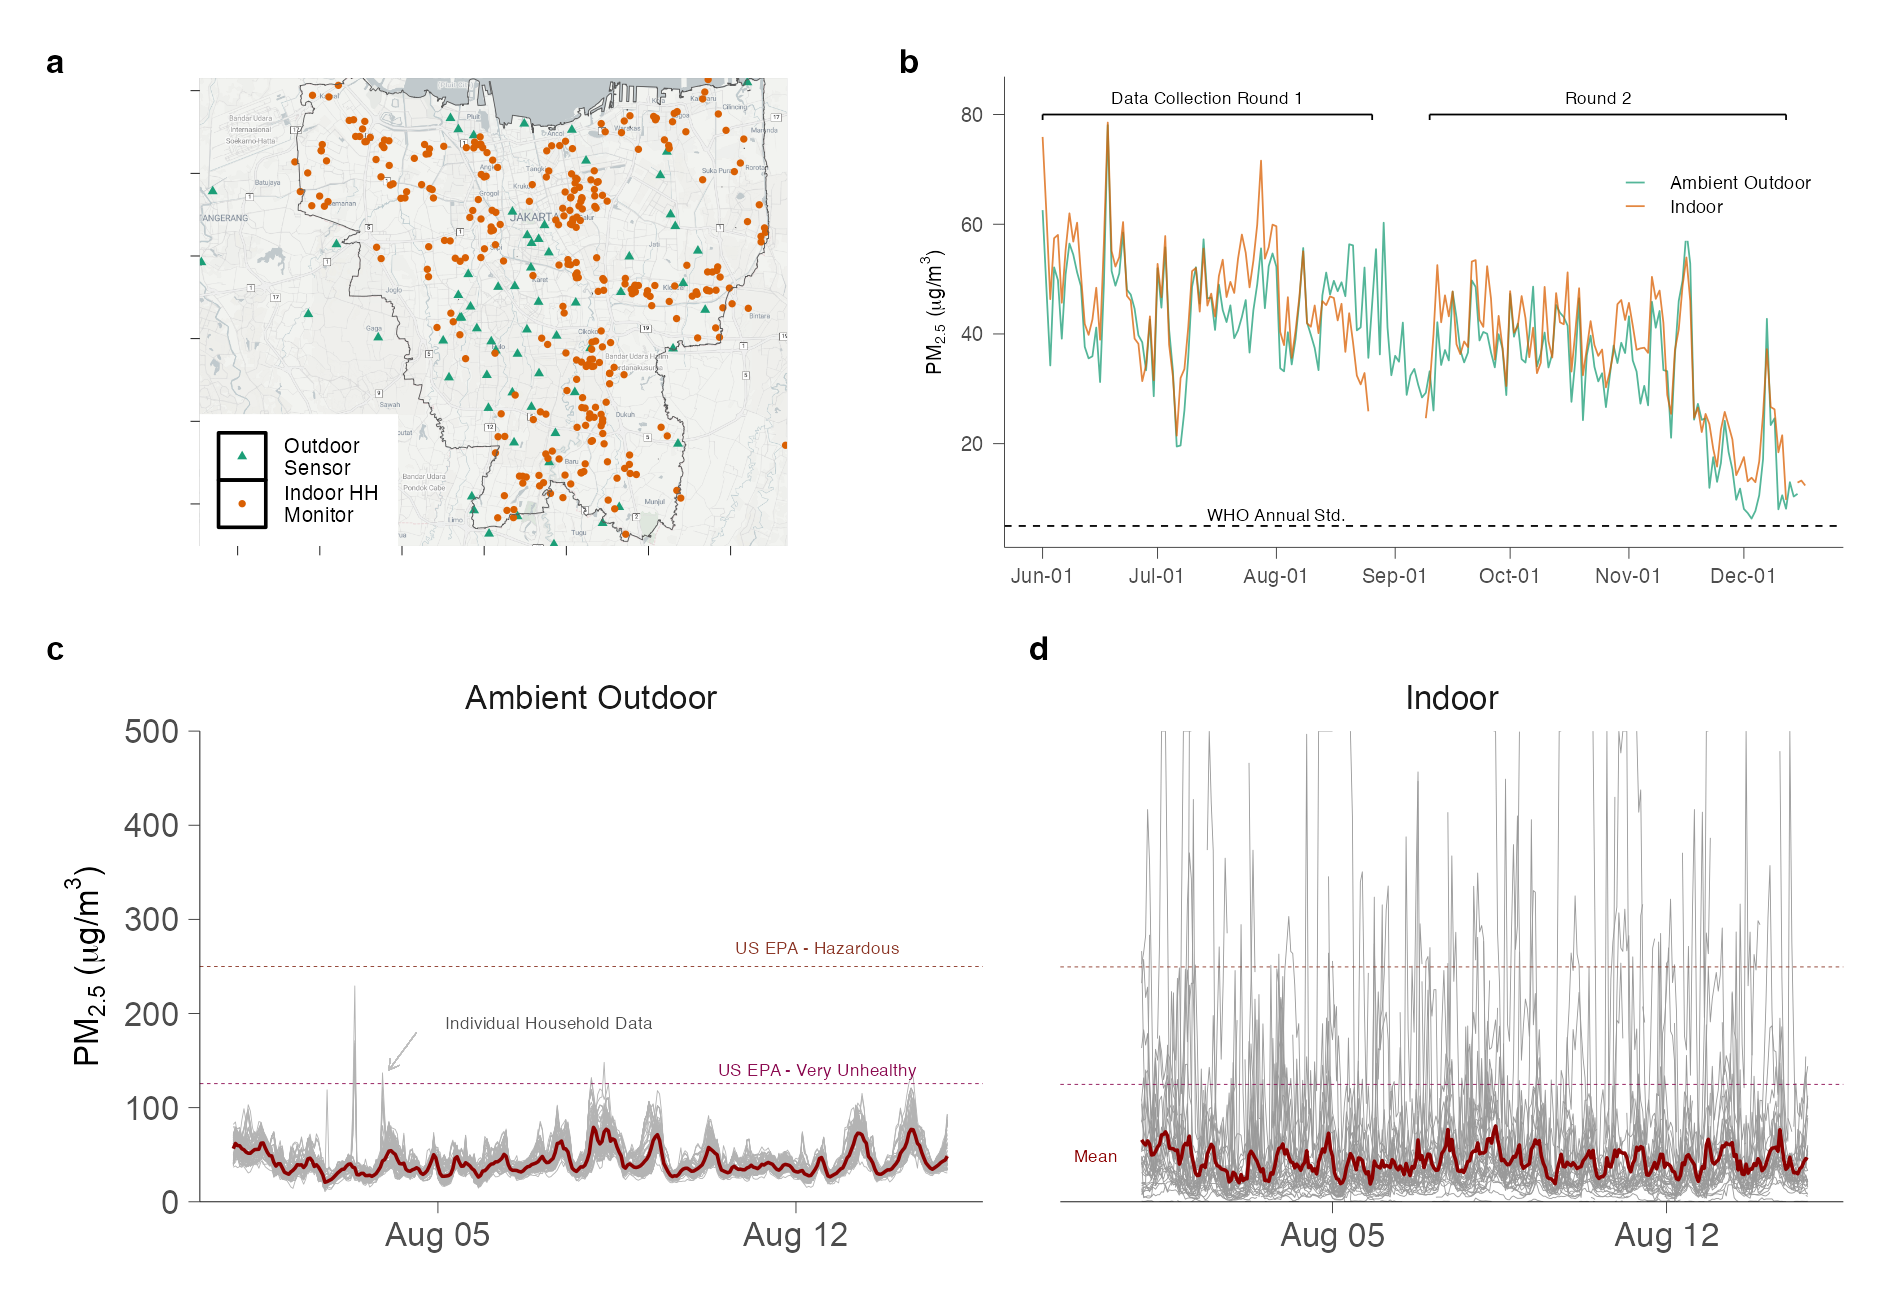
\includegraphics[width=\linewidth]{output_indooroutdoor/desc/fig1_desc.png}
    \caption*{\scriptsize \textbf{(a)} Locations of respondents and installed air quality monitoring hardware. There are 308 indoor air quality monitors (orange) installed in respondent homes, and 63 low-cost sensors (green) to measure respondent-specific outdoor air quality. \textbf{(b)} Daily average outdoor and indoor pollution levels in Jakarta. To account for the uneven spatial distribution of outdoor sensors, we first computed district-level averages for outdoor readings, which were then aggregated to produce a daily citywide average. Indoor pollution levels were averaged across all households on a daily basis. The gap in the indoor data from August 26 to September 8 occurred during a transition period when the air quality hardware was being moved between households. \textbf{(c)} Hourly outdoor $PM_{2.5}$
    from August 1–14, 2024. Gray lines show hourly $PM_{2.5}$ concentrations for each individual low-cost sensor, while the maroon line shows the mean concentration across all 68 sensors. \textbf{(d)} Analogous to (c), this plot shows hourly indoor $PM_{2.5}$.}
    \label{fig:desc_pm}
\end{figure*}

Our main finding is that average indoor $PM_{2.5}$ concentrations closely map ambient outdoor $PM_{2.5}$ concentrations on average, but episodic spikes of indoor $PM_{2.5}$ are often much higher than those outdoors. %Overall, this implies that households are on average exposed to higher levels of $PM_{2.5}$ indoor than outdoor in Jakarta.
Overall, these patterns imply that in Jakarta, households are exposed to higher levels of $PM_{2.5}$ indoors than outdoors on average.

% Similar high levels of indoor / outdoor
We first establish that both indoor and outdoor $PM_{2.5}$ concentrations are at unhealthy levels. During our study period, the mean indoor daily $PM_{2.5}$ concentration was 40.7 $\mu g/m^3$, while the mean outdoor daily $PM_{2.5}$ concentration was 37.8 $\mu g/m^3$. Both levels were about eight times higher than the WHO annual standard of 5 $\mu g/m^3$, as shown on Figure \ref{fig:desc_pm}.

% In addition indoor has spikes
In addition to persistently high pollution levels, we find that indoor spaces also experience severe episodic pollution events. Figure \ref{fig:desc_pm}d displays hourly indoor pollution levels at the individual household level for a representative two-week period from our sample. The figure shows frequent spikes in indoor pollution, soaring far beyond levels characterized as hazardous by the US EPA and surpassing thresholds typically associated with emergency conditions. On average, indoor air exceeds US EPA's ``Very Unhealthy" threshold 4\% of the time—levels that are rarely observed in the outdoor measurements. 


% These indoor spikes matter to the extent people spend time indoor
In our accompanying survey, we find that respondents—90\% of whom were women—reported spending 80\% of their time at home. We focused on parents of elementary school children, who reported that their children spent an average of 70\% of their time indoors. Thus, indoor pollution levels are highly representative of overall $PM_{2.5}$ exposure for women and children in our study population. Importantly, the sample targets low- and middle-income households, offering rare insights into a population largely overlooked in existing research on indoor air quality. Existing research on indoor pollution predominantly examines households in high-income countries \citep{krebs_using_2021, lunderberg_assessing_2023, burke_exposures_2022} or relies on small samples observed over short periods of time \citep{lim_comparing_2022}, leaving significant gaps in our understanding of indoor air pollution exposure in developing urban settings. More details on our sampling approach are provided in Section \ref{ssec:mehtods_sampling}.


Overall, these findings reveal that while outdoor levels capture average indoor exposure, they fail to account for the pollution burden from episodic indoor spikes. Individuals with similar average exposures may experience very different intensities and frequencies of severe pollution events—patterns that are missed when relying solely on outdoor pollution data. The health impacts of repeated short-term spikes remain poorly understood, underscoring the need for research that considers pollution spikes, not just average levels.
%with children spending 70\% of their time at home. Sample with at least one elementary school-aged child
\subsection{Outdoor Infiltration into Indoor Spaces}
\label{ssec:infiltration}

\begin{figure*}[!t]
    \centering
    \caption{Infiltration Rate from Ambient Outdoor to Indoor Homes}    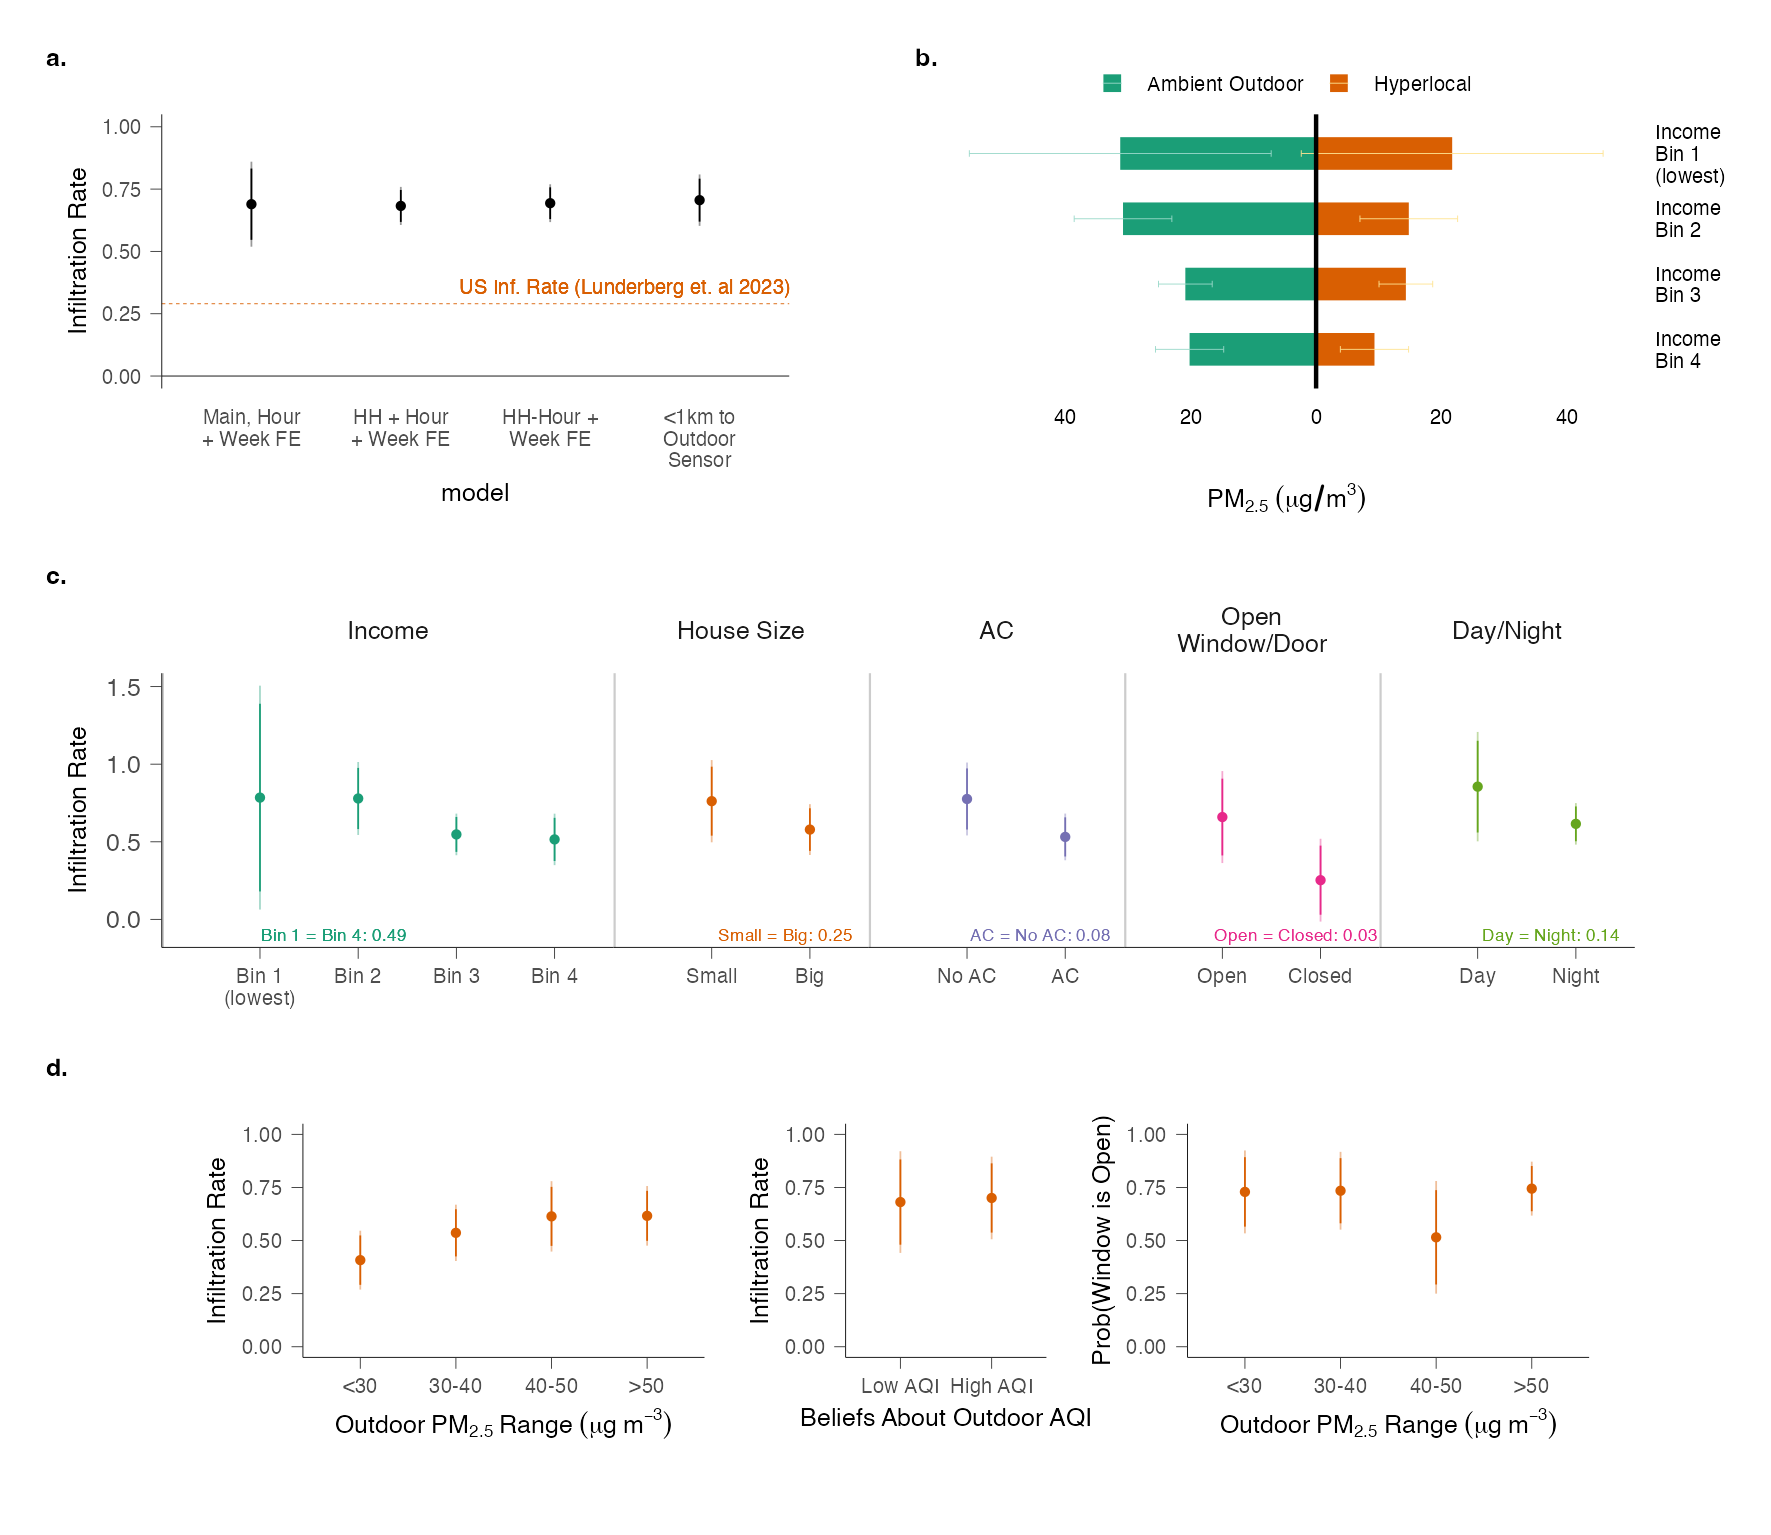
\includegraphics[width=.8\linewidth]{output_indooroutdoor/infiltration/fig3_infiltation.png}
    \caption*{\scriptsize \textbf{(a)} Infiltration rates, defined by the regression  of indoor \( PM_{2.5} \) on outdoor \( PM_{2.5} \). Each point corresponds to a different regression specification. The first specification controls for hour-of-day and week fixed effects, the second adds household fixed effects, and the third further restricts the sample to households located within 1 km of an outdoor sensor. All regressions control for outdoor temperature and humidity.  \textbf{(b)} Decomposition of \( PM_{2.5} \) sources into ambient outdoor and hyperlocal contributions. The ambient outdoor contribution is calculated by multiplying infiltration rates (from the main regression specification in panel a) by the mean outdoor \( PM_{2.5} \). The hyperlocal source is computed by subtracting the outdoor contribution from the total measured indoor \( PM_{2.5} \). Error bars reflect standard errors based on infiltration rates and are scaled by the mean \( PM_{2.5} \) for each quartile,  thus the breakdown should be interpreted as source contribution conditional on the mean $PM_{2.5}$. \textbf{(c)} Heterogeneity in infiltration rates by household and behavioral characteristics, including income quartile, number of rooms in the house (including bathrooms), air conditioning (AC) presence, whether a window/door was open in the room, and time of day (day/night). P-values for tests of equality between coefficients are shown in the respective graphs. \textbf{(d)} Household behavior in response to outdoor pollution levels. The first panel shows the heterogeneity in infiltration rate as a function of outdoor $PM_{2.5}$ concentrations. The second panel shows heterogeneity in infiltration rates based on households’ beliefs about outdoor air quality, comparing those who perceive it as generally unhealthy (high AQI) versus those who do not (low AQI). The third panel regresses the probability of opening windows or doors on outdoor levels.  Points represent regression coefficients; darker error bars show 90\% confidence intervals, and lighter error bars show 95\% confidence intervals. Errors are clustered at the household level.}
    \label{fig:infiltration}
\end{figure*}
We model how ambient outdoor $PM_{2.5}$ infiltrates into indoor spaces; this decomposes the contributions of ambient outdoor sources versus hyperlocal sources to indoor pollution. Ambient outdoor refers to background $PM_{2.5}$ concentrations measured by our citywide sensor network, while hyperlocal sources—including smoking and neighborhood burning—occur at spatial scales too fine for our outdoor sensors to capture.

We estimate that a 1 $\mu g /m^{3}$ increase in ambient outdoor $PM_{2.5}$ is associated with a .689 (95\% CI, 0.508, 0.871; $P < 0.001$) $\mu g /m^{3}$ increase in indoor $PM_{2.5}$ in the same hour. This rate is about 2.5 times the rate typically estimated in the United States \citep{lunderberg_assessing_2023}, consistent with indoor spaces in low- and middle-income countries not offering the same protection from outdoor pollution as in high-income countries. In addition, we find that infiltration happens much more quickly than in high-income settings. We estimate that all infiltration happens within the hour, as opposed to estimated lagged effects up to 6 hours in high-income settings \citep{burke_exposures_2022, lunderberg_assessing_2023}. These estimates are robust to alternative regression models, as seen in Figure \ref{fig:infiltration}a. 

As a result of these high infiltration rates, most indoor air pollution in Jakarta originates from the outdoors—unlike in high-income countries, where indoor pollution typically stems from indoor sources \citep{metcalfe_making_2025}. Overall, we estimate that 63\% of mean indoor PM2.5 comes from ambient outdoor pollution (Figure \ref{fig:infiltration}b).


To shed light on the causes behind these high infiltration rates, we examine heterogeneity in infiltration rates in Figure \ref{fig:infiltration}c. We find statistically significant differences based on air conditioning (AC) ownership (p = 0.08) and whether the monitor room has an open versus closed window or door (p = 0.03). These findings corroborate ventilation as a key determinant of infiltration rates. In Jakarta’s hot and humid climate, households without AC often rely on natural ventilation, increasing their exposure to outdoor pollution. 

Our results suggest that differences in infiltration rates are driven by long-term household characteristics. This is in contrast to previous studies in high-income settings finding that infiltration rates are primarily driven by short-term behavioral adjustments \citep{burke_exposures_2022, baquie_know_2024}. We conduct three analyses to show that  households are not actively taking short-term actions to reduce infiltration.

First, while previous literature has found that infiltration rates decline at high outdoor $PM_{2.5}$ concentrations, suggesting that people actively modify their behavior to limit exposure at higher levels of outdoor pollution \citep{burke_exposures_2022,lunderberg_assessing_2023}, we do not find evidence of this relationship in our setting. In fact, infiltration increases at higher $PM_{2.5}$ concentrations. This pattern, shown in Figure \ref{fig:infiltration}d, could be driven by several factors, including concentration gradients between outdoor and indoor pollution, meteorological conditions correlated with outdoor pollution levels, or the presence of high-emission hyperlocal pollution sources \citep{lunderberg_assessing_2023,macneill_factors_2012}.

Second, we assess whether ventilation behaviors (e.g., opening windows or doors) respond to outdoor pollution levels. If households actively manage infiltration, we would expect them to close windows when pollution is high. However, Figure \ref{fig:infiltration}d shows no relationship between window or door openness and outdoor pollution levels. While opening or closing windows is a short-term behavior that can, in theory, be adapted, it is difficult to expect households to keep windows closed in a hot and humid climate like Jakarta, where natural ventilation is important for cooling. 

Finally, we find no evidence that beliefs translate into meaningful protective action. Infiltration rates do not differ between households who perceive outdoor air as unhealthy and those who consider it relatively healthy, as shown in Figure \ref{fig:infiltration}d. Households were classified based on whether they generally thought outdoor air pollution was unhealthy (high AQI vs. low AQI) before monitors were installed. The disconnection between beliefs and protective action is consistent with other research finding low protective behavior in low-income settings \citep{greenstone_indoor_2021, chowdhury_misbeliefs_2025}.



\subsection{Hyperlocal Sources of Indoor $PM_{2.5}$ Spikes}
While ambient outdoor pollution is the primary driver of persistently high indoor $PM_{2.5}$ concentrations, we find that hyperlocal sources are responsible for the episodic spikes that lead to extreme pollution levels. Our surveys, as shown in Figure \ref{fig:hyperlocal_sources}, clearly document the impact of two major sources: indoor smoking and neighborhood waste burning.\footnote{It is worth noting that another major contributor to indoor air pollution that has been documented extensively is the combustion of solid fuels and kerosene for cooking. However, in Indonesia, the widespread adoption of LPG cookstoves has largely eliminated variation in cooking fuel use \citep{astuti_successful_2019}; in our survey, 98\% of households reported using LPG cookstoves for cooking. While LPG cookstoves still generate large spikes in pollution, our data do not include detailed information on cooking activities, preventing us from drawing insights on this source of indoor pollution.}


\begin{figure*}[!t]
    \centering
    \caption{Contributions of Hyperlocal Pollution}
    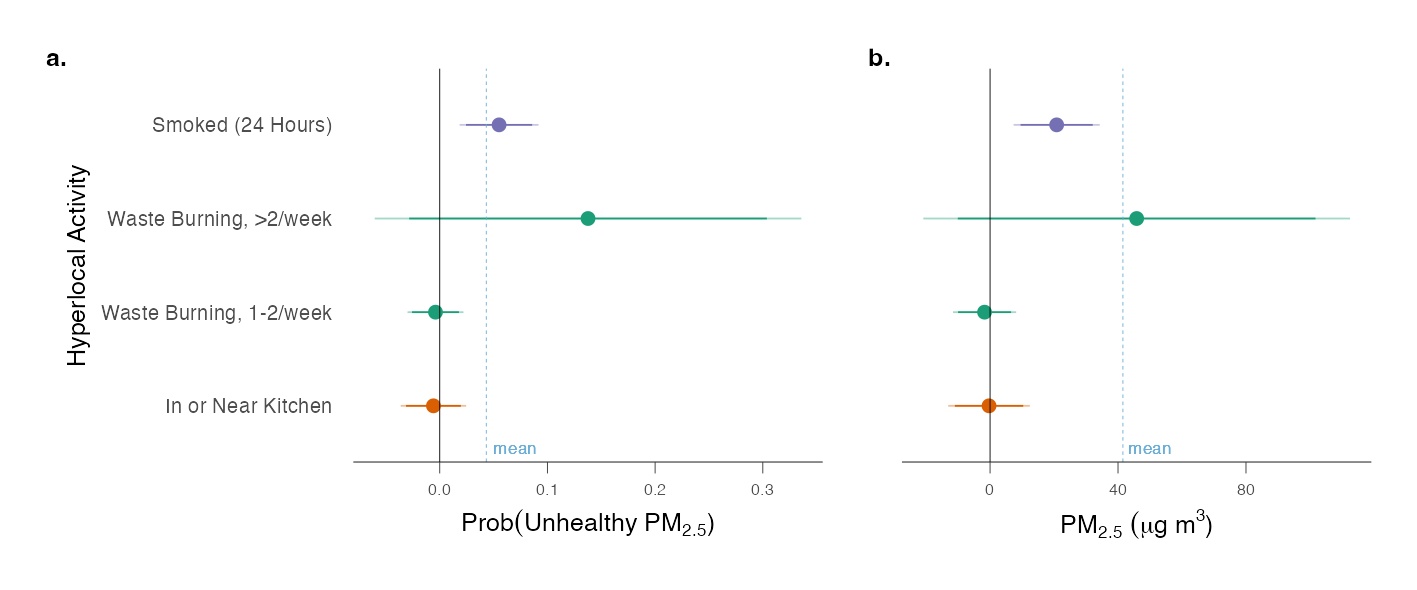
\includegraphics[width=.8\linewidth]{output_indooroutdoor/infiltration/fig4_hyperlocal.png}
    \caption*{\scriptsize \textbf{(a)} Regression coefficients for the probability that $PM_{2.5}$ exceeds the EPA's AQI threshold for very unhealthy levels (greater than 125 $\mu g / m^3$) as a function of indoor pollution-generating activities: (1) whether the monitor is in or near the kitchen, (2) whether the households reported observing 1-2 waste burning events in the neighborhood in the 7 days preceding the interview, (3) whether the household reported observing more than 2 waste burning events in the neighborhood in the 7 days preceding the interview, and (4) whether the household reported any smoking indoors in the 24 hours preceding the interview.  
    \textbf{(b)} Analogous to panel (a), this panel shows regression coefficients of indoor $PM_{2.5}$ concentrations on indoor pollution-generating activities.  
    Points represent regression coefficients; darker error bars show 90\% confidence intervals, and lighter error bars show 95\% confidence intervals. Errors are clustered at the household level. The light blue dashed line shows the sample mean for each respective measure of indoor pollution.}
    \label{fig:hyperlocal_sources}
\end{figure*}

We find that households who reported indoor smoking within the last 24 hours experienced significantly higher indoor pollution levels. These households had a 5.51\% (95\% CI: 1.85–9.17, $P < 0.001$) greater probability of pollution spikes reaching very unhealthy levels. Given that the sample average probability of pollution spikes is 4.43\%, this corresponds to a 127\% increase. Analogously, smoking was associated with 20.8 $\mu g/m^3$ (95\% CI: 7.36–34.3, $P < 0.001$) higher average hourly indoor $PM_{2.5}$ concentrations, a 50\% increase compared to the sample mean.

Neighborhood-level waste burning is another significant source of indoor air pollution in Jakarta. Households in areas with more than two waste-burning events per week experienced notably higher indoor $PM_{2.5}$ concentrations. However, accurately quantifying the effect of burning events on indoor pollution is challenging because we rely on self-reported data and some events may be misreported. These measurement limitations contribute to wide confidence intervals around our estimates.

In addition to smoking and neighborhood waste burning, there are likely other hyperlocal pollution sources contributing to the observed spikes in indoor air pollution. Such activities may include cooking, traffic emissions, industrial operations, and commercial activities. An exhaustive list of all polluting activities is beyond the scope of our analysis.

%We also estimate infiltration rates separately for each income quartile to assess how much of indoor $PM_{2.5}$ originates from outdoor sources. Figure \ref{fig:infiltration}b shows that across all income quartiles, the majority of indoor $PM_{2.5}$ comes from outdoor sources (59–68\%). While point estimates suggest some differences across income groups, large confidence intervals caution against overinterpreting these differences.


%\subsection{Income is a Major Driver of Heterogeneity in Exposure to Indoor $PM_{2.5}$}
\subsection{Heterogeneity by Income}

Households across the income distribution experience similar levels of ambient outdoor pollution exposure, but lower-income households suffer higher levels of indoor $PM_{2.5}$. As shown in Figure \ref{fig:pm_income}a, moving from the highest to the lowest income quartile in our sample is associated with an increase of 23.4 $\mu g/m^3$ in mean $PM_{2.5}$, representing a 79\% increase. This finding is consistent across various aggregation techniques used to calculate the mean (SI Appendix, Figure A2).

\begin{figure*}
    \centering
    \caption{Indoor $PM_{2.5}$ Higher for Lower Income Households}
    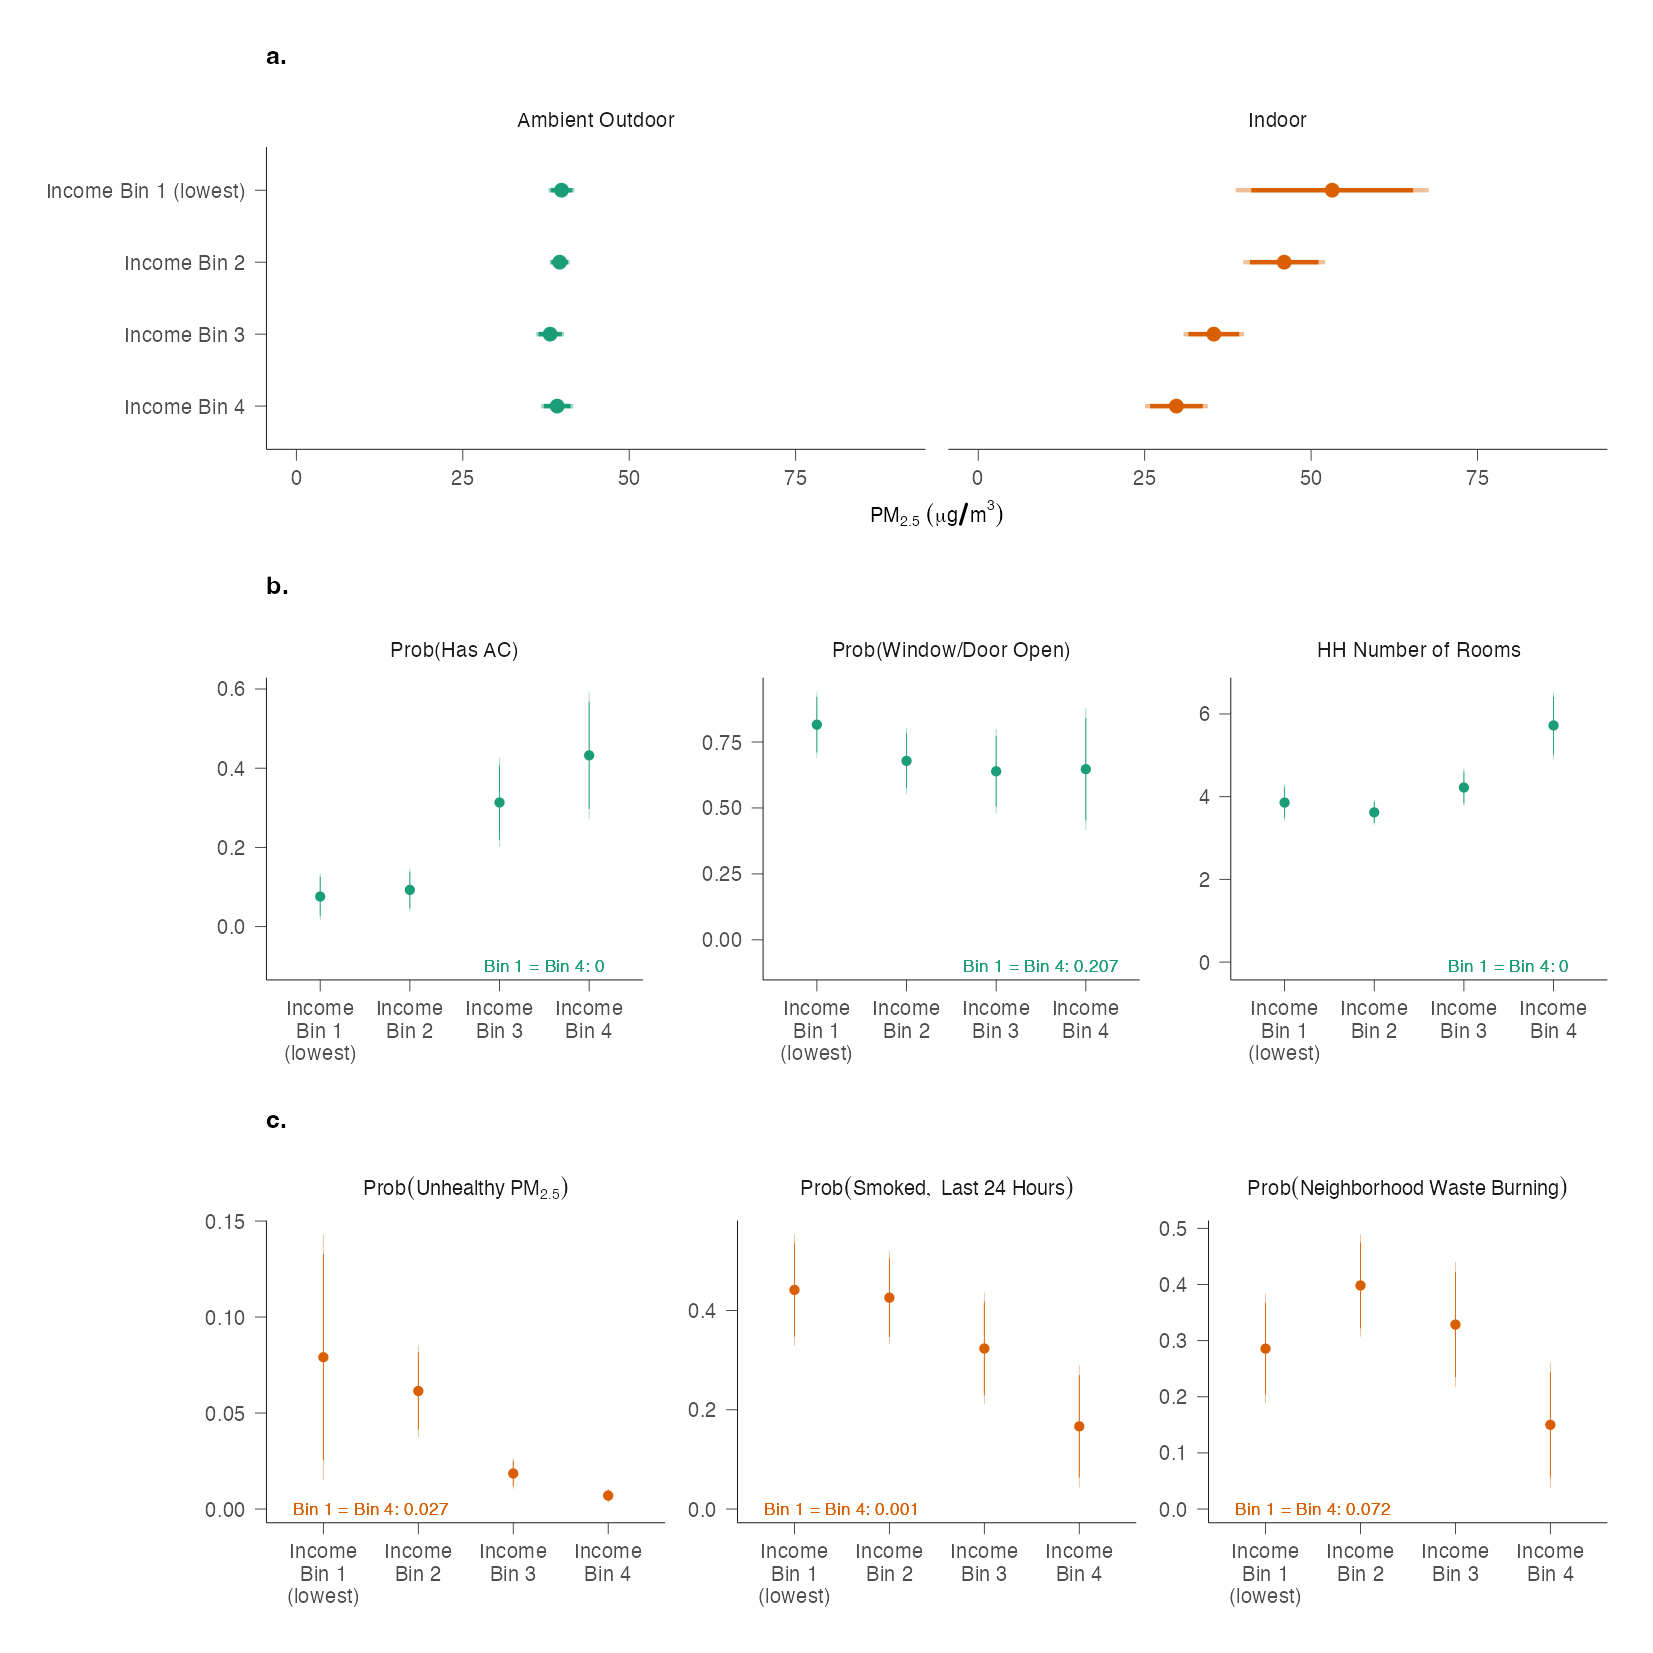
\includegraphics[width=\linewidth]{output_indooroutdoor/desc/fig2_pm_income.png}
    \caption*{\scriptsize  \textbf{(a)} Mean $PM_{2.5}$ concentrations across income quartiles for indoor and ambient outdoor measurements. For ambient outdoor measurements, a household-hour level weighted average was calculated using air quality readings from the three nearest sensors, with weights inversely proportional to distance. A mean level was then computed for each household, followed by aggregation across households within each income quartile. Indoor $PM_{2.5}$ measurements were aggregated similarly, starting with household-level means and then averaging across households within each income quartile. \textbf{(b)} Regressions of household  characteristics related to outdoor infiltration by income quartile, with Income Bin 1 as the lowest income. Panels show regression coefficients where outcome variable is number of rooms, whether household has air conditioning, and whether windows/doors were open when surveyed. Points represent estimated regression coefficients; darker error bars show 90\% confidence intervals, and lighter error bars show 95\% confidence intervals. Standard errors are clustered at the household level. P-values for tests of equality between coefficients are shown in the respective graphs.
    \textbf{(c)} Similar to (b), regressions of characteristics linked to hyperlocal pollution sources on income quartile. 
    The first panel is the probability that hourly $PM_{2.5}$ exceeds the EPA's AQI threshold for very unhealthy levels (greater than 125~$\mu g / m^3$) on income quartile, controlling for outdoor pollution, temperature, humidity, week, and hour-of-day fixed effects. Income Bin 1 (lowest income) is the reference group. The second regresses the indoor smoking in the last 24 hours on income quartile. The third panel regresses whether there was more than 2 waste burning activities reported that week in the neighborhood on income quartile. Points represent estimated regression coefficients; darker error bars show 90\% confidence intervals, and lighter error bars show 95\% confidence intervals. Standard errors are clustered at the household level. P-values for tests of equality between coefficients are shown in the respective graphs.
}
    \label{fig:pm_income}
\end{figure*}

Indoor air quality is determined by how much outdoor $PM_{2.5}$ infiltrates indoors and how much pollution is generated hyperlocally. We find that income affects both these factors. 

Income may affect infiltration of outdoor pollution into indoor spaces through its impact on housing quality and ventilation choices \citep{lunderberg_assessing_2023}. In Jakarta’s hot and humid climate, households may cool indoor spaces through either air conditioning or natural ventilation. As shown in Figure \ref{fig:pm_income}b, higher-income households are significantly more likely to have air conditioning, reducing their reliance on open windows or doors for ventilation. Consistent with this pattern, households in the lowest income quartile are more likely to keep windows or doors open in the air quality monitor room at the time of surveying, although this difference is not statistically significant. Higher-income households also tend to live in larger homes, potentially enabling them to separate living areas from cooking and smoking areas, for example. Taken together, these patterns are consistent with lower-income households having lower housing quality and facing greater challenges in regulating indoor temperatures, making them more vulnerable to outdoor pollution infiltration, as discussed in Section \ref{ssec:infiltration}.

Income is also closely linked to hyperlocal pollution sources shaped by household and neighborhood behaviors. We proxy for exposure to hyperlocal sources by the likelihood that mean hourly $PM_{2.5}$ exceeds the EPA's AQI threshold for very unhealthy levels ($125~\mu g / m^3$). Since ambient outdoor pollution rarely reaches such extreme levels in Jakarta, these spikes likely result from episodic emissions occurring inside or near the home. 
%
As shown in Figure \ref{fig:pm_income}c, households in the lowest income quartile experience unhealthy pollution spikes 10.5\% of the time, compared to just 3.23\% in the highest income quartile. A statistical test of the difference in coefficients between the lowest income quartile and the highest quartile confirms that this difference is statistically significant ($p = 0.027$). This disparity suggests a greater burden of episodic pollution for low-income households.
%
We further examine the relationship between income and two prominent hyperlocal pollution sources: indoor smoking and neighborhood waste burning. Indoor smoking is significantly less common among higher-income households, as shown in Figure \ref{fig:pm_income}c. Waste burning, another potential contributor, does not follow a clear income gradient, though measurement challenges limit the robustness of this finding.\footnote{As previously mentioned, the combustion of solid fuels and kerosene for cooking has previously been documented as another major contribution to indoor air pollution. However, the widespread adoption of LPG cookstoves has largely eliminated variation in cooking fuel use and the absence of details on cooking activities in our data prevent us from further investigating the role of cooking on air pollution.
}




\section{Discussion}

We show that indoor $PM_{2.5}$ exposure in Jakarta is both persistently high and unequally distributed across income groups. In addition to elevated average levels, indoor environments frequently experience hazardous pollution spikes—extremes not captured by outdoor monitors. These spikes occur despite 98\% of households in our sample using LPG cookstoves—a fuel typically classified as clean cooking. This highlights the need for a broader framework for understanding indoor air pollution in low- and middle-income countries.
For example, the Global Burden of Disease (GBD) framework defines household air pollution in terms of solid fuel use—a metric that has guided policy and resource allocation globally. However, this definition does not fully capture the indoor pollution risks experienced by urban populations that use cleaner fuels but remain exposed to high ambient and infiltrated pollution. 

We find that most indoor pollution stems from outdoor $PM_{2.5}$ infiltration, with an infiltration factor (0.689) substantially higher than estimates in high-income countries. These high rates are related to structural characteristics, such as the absence of air conditioning and the dependence on natural ventilation, rather than short-term behavioral responses. While information campaigns may increase awareness of infiltration risks, economic and infrastructural constraints likely limit behavioral adjustments. Mitigation efforts must therefore prioritize  pollution controls at the source, targeting major contributors like vehicular traffic and industrial emissions. In the interim, coupling outdoor air quality mapping with demographically representative indoor measurements can help better characterize true exposure and inform more equitable policy design.


In contrast, episodic peaks in indoor pollution are driven by hyperlocal sources such as indoor smoking and neighborhood waste burning, activities more amenable to individual or local intervention. Information campaigns and stronger enforcement against garbage burning could reduce these extreme events and their associated health risks.


Our findings also have important distributional implications. Consistent with previous studies \citep{greenstone_indoor_2021, burke_exposures_2022, ito_willingness_2020}, we show that low-income households are exposed to the highest levels of indoor air pollution. Relying solely on outdoor air quality as a proxy for exposure may systematically underestimate both overall exposure and disparities across income groups. These inequalities stem from both higher infiltration rates, associated with poorer housing conditions, and greater hyperlocal emissions. 


Finally, while our study provides novel insights into indoor $PM_{2.5}$ exposure in a developing urban setting, it has several limitations. First, our sample focuses on  households with elementary school-aged children, and therefore is not fully representative of Jakarta’s population. Future research should assess whether similar patterns hold for other demographic groups, particularly groups with heightened health risks, such as the elderly or those with pre-existing health conditions. Second, while we identify key determinants of indoor air quality, we do not capture all possible hyperlocal pollution sources, such as cooking emissions, incense burning, or traffic-related infiltration, nor are we able to track personal exposure outside the home. Relatedly, our reliance on stationary indoor monitors limits our ability to account for variations in individual exposure as people move between environments. Expanding real-time monitoring to include wearable sensors and more detailed measurements of indoor pollution sources could provide a fuller picture of exposure risks.

\section{Materials and Methods}
High levels of outdoor air pollution are sustained in Jakarta throughout the whole year, and historically especially high between the months of May and October. We designed the study to cover this high pollution season and conducted it in two successive rounds, with approximately 154 households participating in each round. Round 1 was conducted from 1 June to 28 August 2024, and Round 2 was conducted from 10 September to 10 December 2024. This randomized controlled trial was registered on the AEA RCT registry (Identification No. AEARCTR-0013110) and received IRB approval from the University of Chicago (Protocol No. IRB23-0310) and from Badan Riset dan Inovasi Nasional (Application No. 29012024000032).
% DATA
Individual respondents consented to the collection of the indoor air quality data and survey data used in this study. Ambient outdoor $PM_{2.5}$ data comes from devices monitored by our hardware implementation partner, not associated with private individuals, and therefore without personally identifying information.


\subsection{Study Participants and Datasets}
\label{ssec:mehtods_sampling}

\paragraph{Study Participants:} Households participating in our study were selected among Jakarta households, through a partnership with the Education Office in Jakarta, which compiled a representative list of Jakarta schools. We randomly sampled households from school rosters and successfully enrolled 308 participants, 285 of whom successfully installed the hardware, connected to Wi-Fi, and operationalized the devices for data collection. Therefore, all our participant households have at least one elementary school child. As surveying challenges like low participation and high attrition are common in developing country cities \citep{greenstone_indoor_2021}, our sample strategy was designed to address these challenges and ensure the proper use and return of air quality hardware. By the end of our study, attrition was only 6\%. This attrition rate is consistent with rates typically observed in rural contexts, but is an exceptionally low rate for surveying in urban settings. For instance, \citep{greenstone_indoor_2021}, a paper with a similar research question conducted in Delhi, reported attrition rates of 19–32\% across their treatment groups. All analyses were conducted in R version 4.3.2.

Figure \ref{fig:desc_pm}a displays the geographic distribution of participating households and demonstrates the wide coverage across the city. Households in our sample are relatively larger and less wealthy than the average Jakarta household but span a wide range of socio-economic backgrounds. For more information on how our sample compares to the wider Jakarta population, see SI Appendix, Table A2.

Following enrollment, the survey enumerators visited households to obtain informed consent and administer a baseline survey. This survey captured household demographic information, housing structure characteristics, and beliefs and behaviors related to indoor and outdoor air pollution. Upon consent, air quality hardware was installed in the home for approximately three months, during which it collected continuous indoor air quality data. Survey questions are listed in the SI Appendix.

\paragraph{Indoor $PM_{2.5}$:} The air quality hardware consisted of a fan equipped with an internal $PM_{2.5}$ sensor (Cubic PM2008M) and was installed in each participating household. The sensor measures particulate concentration via an optical light-scattering method, with accuracy specifications based on factory calibration against a GRIMM aerosol spectrometer. The sensors were designed to collect $PM_{2.5}$ data in real time, with readings not visible to respondents. When connected to Wi-Fi, the devices transmitted data to a remote server at five-minute intervals, which were subsequently aggregated to the hourly level for analysis. The hardware was produced by Nafas, a Jakarta-based air quality technology company. 

To incentivize households to keep the hardware on, participants received IDR 35,000 (approximately USD 2) every 30 days, contingent on the hardware being connected to Wi-Fi and operational for an average of 14 hours per day. For households without Wi-Fi or unwilling to use their Wi-Fi for the experiment, dedicated Wi-Fi units were installed. To offset electricity costs, participants received an additional IDR 15,000 (approximately USD 1) every 30 days.

\paragraph{Outdoor $PM_{2.5}$:} Our hardware partner, Nafas, maintains a dense network of low-cost Airly outdoor sensors across the city, each equipped with a Plantower PMS5003 optical light-scattering sensor. Accuracy and network performance follow the manufacturer’s factory calibration and Nafas’s routine QA/QC procedures. For each household, we calculate a weighted average of air quality readings from the three nearest outdoor sensors, assigning weights inversely proportional to the distance to each sensor. The 63 outdoor sensors used in this study also capture temperature and humidity data, which we use as controls. The outdoor low-cost sensors were installed prior to our study and were not randomly distributed across space, which could introduce non-randomly distributed measurement error. We test for selection in the location of outdoor sensors by regressing a household's distance to the closest outdoor sensor on recorded indoor $PM_{2.5}$, recorded outdoor $PM_{2.5}$ of this sensor, household income, house size, whether the household owns an AC, household head employment status, and household head education level. We do not find evidence of selection bias on observables, as shown in the SI Appendix, Table A1.

\paragraph{Natural ventilation behaviors:} To complement our main survey efforts, we deployed a short WhatsApp survey to participating households on three separate occasions during the study period. The survey asked respondents whether the windows and doors in the room housing the indoor monitor had been open or closed during the past hour.


\subsection{Infiltration Rate}
The average indoor infiltration rate is defined as the increase in indoor $PM_{2.5}$ concentration per unit increase in local ambient outdoor $PM_{2.5}$ concentration. To estimate this rate, we used a regression model at the monitor-hour level. For each household $i$ in hour $t$, the infiltration rate ($\beta$) was estimated using the following specification:
\iffalse
\begin{align}
\label{eq:infiltration}
    PM^{In}_{it} &= \alpha + \beta PM^{Out}_{it} + \pi T_{it} + \gamma H_{it} + f(i, h, w) + \varepsilon_{it}
\end{align}
\fi
\begin{align}
\label{eq:infiltration}
    PM^{In}_{it} &= \alpha + \beta PM^{Out}_{it} + \pi T_{it} + \gamma H_{it} + \mu_h + \mu_w + \varepsilon_{it}
\end{align}
where $PM^{In}_{it}$ and $PM^{Out}_{it}$ denote indoor and outdoor $PM_{2.5}$ concentrations, respectively. $T_{it}$ and $H_{it}$ are controls for contemporaneous outdoor temperature and humidity. Hour-of-day controls $\mu_h$ capture diurnal patterns in pollution and household activities, and week-of-sample controls $\mu_w$ capture temporal trends and broader atmospheric conditions.


Figure \ref{fig:infiltration}a presents the results of this regression model for this main specification and alternative ones: 
\begin{enumerate}
    \item Main specification: includes controls for average variation in $PM_{2.5}$ over the course of the day (hour-of-day fixed effects, $\mu_h$) and average weekly trends (week-of-sample fixed effects, $\mu_w$).
    \item All controls included in specification 1, as well as controls for time-invariant differences across households ($\mu_i$).
    \item All controls included in specification 1, as well as controls for household-specific average variation in $PM_{2.5}$ at different times of the day (household-hour-of-day fixed effects, $\mu_{ih}$).
    \item Specification 1 but restricts the sample to households located within 1 km of a low-cost outdoor sensor to assess the potential impact of measurement error in outdoor $PM_{2.5}$ concentrations on infiltration estimates.
\end{enumerate}

The estimated infiltration rate ($\beta$) remains highly stable across all specifications. We chose specification 1, which includes hour-of-day and week-of-sample fixed effects, as our main specification as it enables us to examine heterogeneity by household-level characteristics, which would not be possible in the presence of household fixed-effects ($\mu_i$). 
\\ 

We further investigate lagged effects of outdoor $PM_{2.5}$ with the following specification:
\begin{align}
     PM^{In}_{it} &= \alpha + \sum_{k = 0}^{11}\beta_k PM^{Out}_{it} + \pi T_{it} \\ &\quad + \gamma H_{it} +\mu_h + \mu_w + \varepsilon_{it} \notag
\end{align}
We present the results when including 11 lags (outdoor $PM_{2.5}$ at each of the previous 11 hours) and ensure that the results are robust to the inclusion of additional lags. From this regression, we derive an estimate of outdoor-indoor infiltration by calculating the cumulative effect of a 1 $\mu g/m^3$ increase in outdoor concentration on indoor concentration:
\begin{align}
    \beta' = \sum_{k=0}^11 \beta_k
\end{align}
Infiltration rates derived from this lagged regression are very similar to our main estimates, consistent with most of the infiltration happening within the first hour, as shown in Figure \ref{fig:infiltration}.
\\

To examine heterogeneity in infiltration rates across household characteristics $X_i$, we run the following interacted specification:
\begin{align}
    PM^{In}_{it} &= \alpha + \beta_1 PM^{Out}_{it} + \beta_2 X_i + \beta_3(PM^{Out}_{it} \times X_i) \\ 
    &\quad + \pi T_{it} + \gamma H_{it} + \mu_h + \mu_w + \varepsilon_{it} \notag
\end{align}

\acknow{We are very grateful to those at SMERU Institute, including Athia Yumna for project guidance; Maudita Dwi Anbarani, Wandira Senja Larasati, Selly Numrala, and Dimitri Swasthika for outstanding project management and field implementation. We are also grateful to Marianne Bertrand, Fiona Burlig, Joshua Dean, and Michael Greenstone for helpful comments and suggestions. We acknowledge Nafas for their role in supplying hardware and outdoor air quality data to this project. This research was funded by the Asian Development Bank Institute, King Climate Action Initiative of the Abdul Latif Jameel Poverty Action Lab (JPAL), Becker Friedman Institute's Weiss Fund and Development Economics Research Fund, Stevens Doctoral Program Office at Chicago Booth, and the Rustandy Center for Social Sector Innovation at Chicago Booth for their generous financial support. The funders had no role in study design, data collection and analysis, decision to publish or preparation of the manuscript. This research has been approved by the Institutional Review Board (IRB) at the University of Chicago (Protocol No. IRB23-0310).}

\showacknow{} % Display the acknowledgments section

\vspace{1cm}
\bibsplit[8]
%Use \bibsplit to split the references from the body of the text. Value "[2]" represents the number of reference in the left column (Note: Please avoid single column figures & tables on this page.)

% Bibliography
\bibliography{JakartaPM}
\end{document}
